% !TEX root = ../../I4PRJ, Grp3 - Rapport.tex
\subsubsection{Implementering}
Implementeringen af iOS-applikationen bestod delvist i den visuelle implementering af brugergrænsefladen, og den kode-mæssige implementering af de bagomliggende view-klasser. Som beskrevet i designafsnittet, implementeres view-klasserne som controller-broer, der implementerer view-interfaces angivet i præsentationslaget. Implementeringen af view-klasserne foretages i udviklingsværktøjet Xamarin, i sproget C\#. 

\paragraph{StatViewBridge.cs}
StatViewBridge implementerer IStatView-interfacet. Klassen skal i følge den tilknyttede user story, vise nyeste måledata. Dette blev løst ved at bruge UIKit-controller klassen UITableViewController, som superklasse. Med få overrides af superklassens metoder, og design af en speciel tabelcelle, kunne data vises dynamisk i view'et. I listing~\ref{code:ios_impl_stattableor} ses override metoden, der sørger for opsætningen af en tabelcelle. Variablen \_sensorData, er data modtaget fra presenter-klassen, ved kald af DisplayCurrentData(...).

\begin{lstlisting}[caption={Override af UITableViewController-metoden GetCell},label={code:ios_impl_stattableor}]
public override UITableViewCell GetCell (UITableView tableView, Foundation.NSIndexPath indexPath)
{	
	var cell = tableView.DequeueReusableCell (_reuseIdentifier) as StatViewCell;
	var type = string.Format ($"{_sensorData [indexPath.Row].Item1}");
	cell.DataLabel.Text = string.Format ($"{_sensorData [indexPath.Row].Item2}") + GuiCharacter.SignForType(_sensorData [indexPath.Row].Item1);
	cell.NameLabel.Text = type;
	cell.BorderImage.Image = UIImage.FromFile (type.ToLower () + ".png");
	return cell;
}
\end{lstlisting}

Ligesom på Windows-platformen, implementeres et view til visning af historisk data også på iOS. HistoryViewBridge er implementeret på samme måde som StatViewBridge, men har også metoder til beregning af graf-punkter. Resultatet af denne implementering ses på figur~\ref{fig:ios_imp_historyview}.

\begin{figure}
\centering
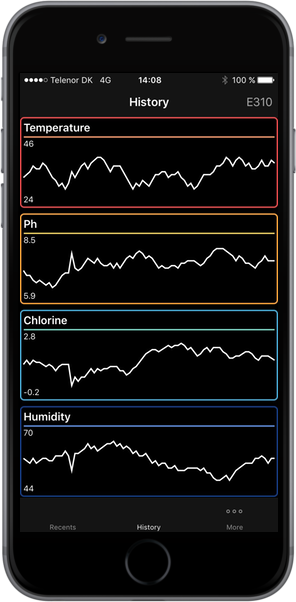
\includegraphics[width=0.4\linewidth]{figs/implementering/ios_imp_historyview}
\caption{Graf vist med HistoryViewBridge på iOS}
\label{fig:ios_imp_historyview}
\end{figure}

For yderligere forklaring se dokumentation afsnit Design under iOS.